% Chapter 2

\chapter{Introduction} % Main chapter title

\label{Chapter2} % For referencing the chapter elsewhere, use \ref{Chapter1} 

\section{Background and Problem Statement}
The biomechanical characterization of soft tissues has gained attention
in medical research \cite{Cox2006}, in areas such as medical image analysis and visualization.
For many years, the obtained medical diagnoses were often based on the assumptions of experts or 
their accumulated experience. While this information have proven to be useful in general, 
these methods have limitations in cases where quantifiable data is necessary, specifically for computer-assisted systems, e.g,
medical diagnosis, therapy, and training \cite{Kauer2002}.
To gather the material data, e.g., elasticity, stiffness, response under deformation and temperature, it is required 
to gain access to the soft tissues and perform in-vivo testing experiments. 
However, obtaining accurate biomechanical data can be challenging 
due to the invasive nature of the procedures and the difficulty in maintaining constant and reproducible internal or external factors  
in experimental configurations \cite{Carter2001}.\\

%Precise knowledge about the biomechanical characterization of soft tissues has received attention
%in medical research, e.g., medical image analysis and visualization.
%For many years, the obtained medical diagnosis have come from assumptions of experts or 
%accumulated experience. This information, although proven to be useful, has its limitations 
%when computed-assisted systems like, medical diagnosis, therapy, and training, rely on 
%more quantifiable data \cite{Kauer2002}. To gather this data, it is important to gain access
%to the tissues and perform in-vivo testing experiments. For organs, this procedure is nearly 
%impossible to achieve, due to the involvement of an invasive procedure, and the lack of constant
%and reproducible external and internal factors. \\ 
Especially, when it comes to internal organs, obtaining reliable data for examination after their 
extraction is difficult because the material properties can vary between samples or testing 
locations on the same organ \cite{Chai2013}. This is due to the influence of various factors such as changes in blood pressure, changes in material properties 
over time, symptoms of disease, and more. In addition, another problem is the lack 
of replication, due to the use of different individuals' organs, which introduces more external
factors into the equation. Moreover, given a tissue sample, it is difficult to properly 
characterize the material due to its anisotropic property, which can lead potentially
 to inaccuracies in the result \cite{Cox2006}.

%Particularly in the case of internal organs, one of the challenges associated with their extraction 
%is that some material properties may change despite examination of the same sample. Their biomechanical properties 
%depend on other factors, such as changes in blood pressure, changes in material properties 
%over time, symptoms of disease, and more. In addition, another problem is the lack 
%of replication, due to the use of different individuals' organs, which introduces more external
% factors into the equation. Moreover, given a tissue sample, it is difficult to properly 
% characterize the material due to its anisotropic property, which can lead to inaccuracies in the result.\\

In the situation where the material data can be collected in a constant, fast and reliable
process, a material model can be established and the computer-aided systems can predict 
the mechanical behavior of soft tissues, providing preoperative calculations. 
This demonstrates the importance of material data collection and material model development, 
especially in the context of computational models such as engineering simulation models created finite 
element analysis (FEA) software and their medical applications in medical devices, surgical 
procedures, and training softwares \cite{Carter2001}. By using accurate material models, the accuracy of the simulation 
can be improved, aiding in a better understanding and predicting a soft tissue response 
to external stimuli \cite{Zhang2014}, making them more useful in medical research and other related applications.\\

\section{Objective and Scope of the Study} 

Soft materials, characterized by low elastic moduli and high sensitivity to external stimuli,
frequently experience large deformation and display nonlinear responses \cite{Zhang2014}, making 
the finite element method (FEM) a common approach for analyzing these materials and solving continuum mechanical problems. 
Although FEM facilitates the analysis of complex structures with complex material 
behavior, simulating such materials requires high computational costs.\\

The main objective of this study is to identify the key parameters of soft materials and their 
influence on the development of a material model based on inverse finite element method (iFEM) approach. 
By identifying these key parameters, an attempt is made to approximate the behavior of 
complex materials through a simplified material model and
assess its potential future applications in medical research and its use with organs.\\

To achieve this goal, an experimental configuration will be selected, and a computational model will be 
developed to use an iFEM approach to identify the key material parameters of the given soft material. 
With this method, it was possible to match the results of the computational model to the experimental 
data, and validate the model with additional data points. 

The objective of this study is to develop a framework that identifies the essential material parameters of soft materials 
and evaluates their limitations and impact on a validated model, which can describe nonlinear material behavior.
By contributing to this framework, the study aims to accelerate the development of material models for practical 
applications in medical research and development.
%---------------------------------------------------------------------------------
\section{State of the Art}

Thi section reviews the state of the art relevant to this study. First, the experimental characterization 
techniques are reviewed, including methods for obtaining mechanical and viscoelastic properties.
This is followed by the description of different approaches to describe the material model for different soft 
materials. Then, the iFEM, which is one method to identify material parameters from experimental data, 
will be explained. Finally, the standard verification and validation process used in computational 
solid mechanics for medical devices based on the American Society of Mechanical Engineering (ASME) guidelines 
will be discussed. The goal of this chapter is to provide a comprehensive overview of the current methods use in 
the field and the identification of limitations and gaps in the current state of knowledge. %maybe take out?

%--------------------------------------------------------------------------------------------------
\subsection{Experimental Characterization for Soft Materials}
\label{subsection:experimentalcharacterization}
%In this section, you can discuss the various experimental techniques that have been used to characterize 
%the mechanical properties of soft materials. You can talk about traditional mechanical testing methods such 
%as tensile and compressive testing, as well as more specialized techniques such as indentation testing, 
%shear testing, and dynamic mechanical analysis. You can also discuss the advantages and limitations of 
%each technique, and highlight any recent advancements in experimental characterization.
%material testing
Experimental testing is a key approach to obtaining information about the mechanical behavior of soft materials.
In order to characterize the mechanical behavior of a test specimen, the most common method
method is to mechanically load the specimen and measure the response of the force against 
the displacement \cite{Bergström2015}. \\


%Soft materials challenges in experimental deign
-Soft synthetics materials like soft gels are often used for tissue engineering applications.
However, due to their 

- Soft synthetics materials like soft gels are one example for soft synthetic materials. These
are commomly applied for tissue engineering applications. Nevertheless, due to their elastic 
modulus range (kPa) present some challenges for the design of experimental testing \cite{Liu2009}.

\subsubsection*{Uniaxial Tension Testing}

Uniaxial tension testing are widely employed to determine an stress-strain relationship.
For uniaxial tension cases, a specimen is typically loaded by gripping the ends while applying 
tension, and the deformation is usually measured with a strain gauge \cite{Bergström2015}.
This kind of testing focuses on the central region of the specimen to evade complication arising from 
"edge effects". An homogeneous deformation in the central region is usually expected for this kind of testing, 
which simplifies the boundary problem and ensures that the measurements represents valid stress-strain values.
However, there are two key limitations for uniaxial testing when testing soft materials; first, 
it may not be suitable when complex boundary conditions arise and is not possible to contro the 
experimental condition entirely \cite{Seshaiyer2003}. Second, these tests are inadequate to 
fully characterize the anisotropic behavior of these materials \cite{Cox2006}.\\

In a study made by Kayanta and Ivankovic (2010), the authors investigated the behavior of an ether-based polyurethane 
elastomer for the creation of mock arteries \cite{Kanyanta2010}. Polyurethane was ideal for this application due to 
its high elasticity and resilience and adaptability to various shapes and sizes. Uniaxial tensile tests on 
dumbbell-shaped specimens were conducted, divided into three groups based on the strain rate.

\begin{figure}
        \centering
    
        \begin{subfigure}[b]{0.45\textwidth}
        \centering
        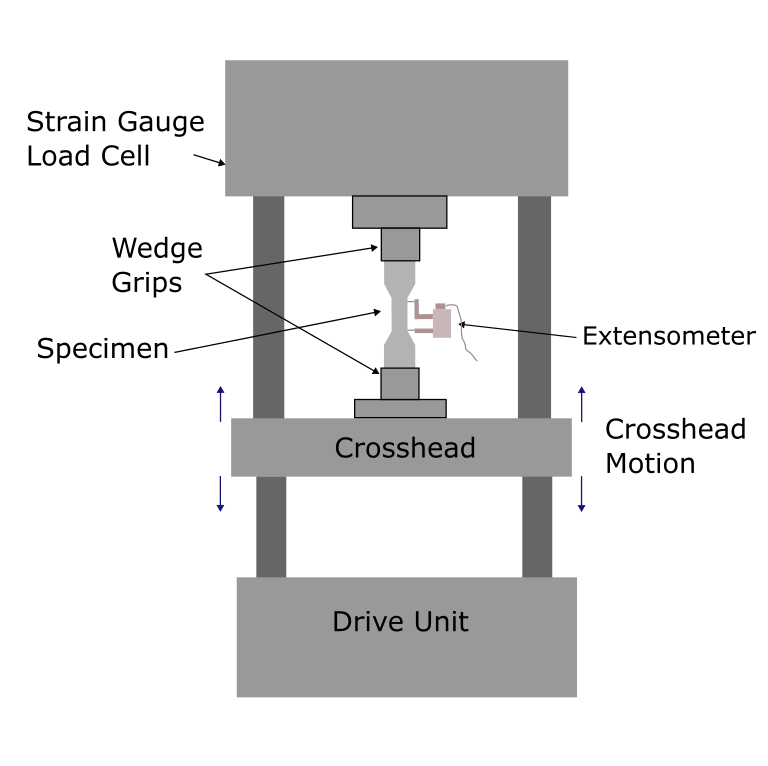
\includegraphics[width=\textwidth]{Images/chapter1/uniaxialtension.png}
        \caption{Low strain rate test with a standard tensile machine}
        \label{fig:subfiglow}
        \end{subfigure}
        \hfill
        \begin{subfigure}[b]{0.45\textwidth}
        \centering
        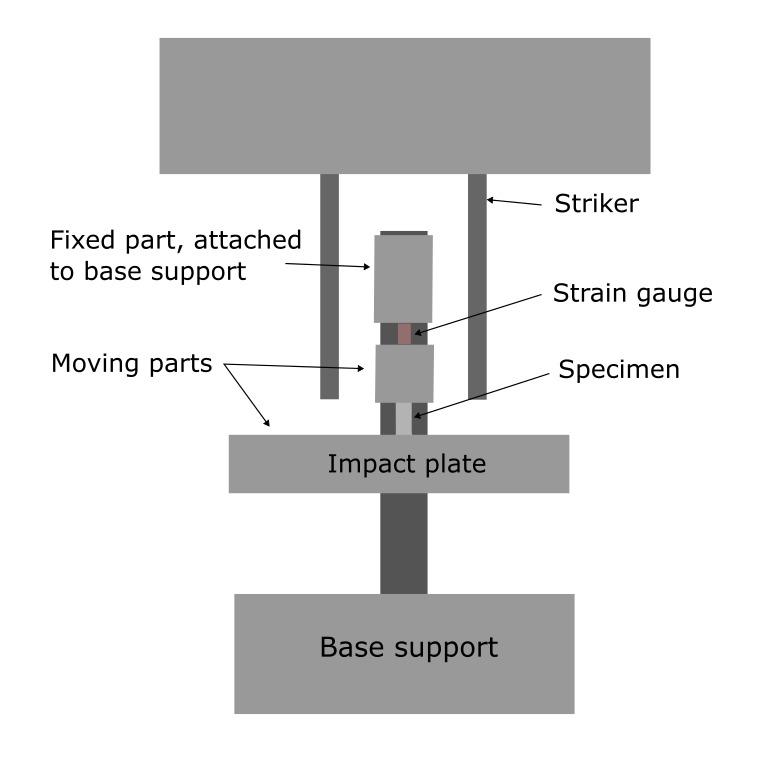
\includegraphics[width=\textwidth]{Images/chapter1/uniaxialintermediate.png}
        \caption{Intermediate strain rate test with a falling weight impact tester}
        \label{fig:subfiginter}
        \end{subfigure}
        \vspace{0.5cm}
        \begin{subfigure}[b]{0.7\textwidth}
        \centering
        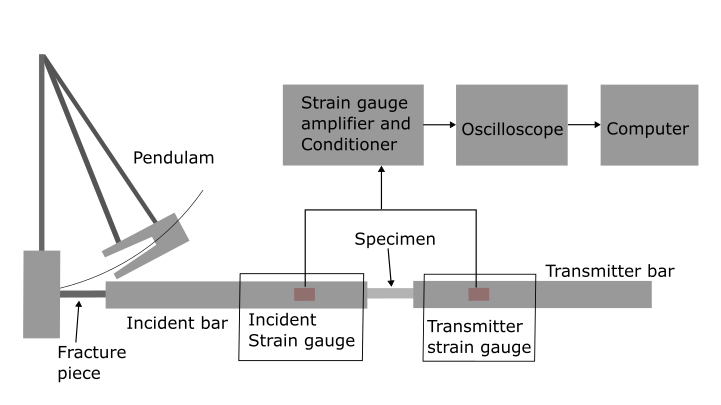
\includegraphics[width=\textwidth]{Images/chapter1/uniaxialhigh.png}
        \caption{High strain rate test with a split Hopkinson pressure bar in tension}
        \label{fig:subfighigh}
        \end{subfigure}  
        \hspace{0.3cm}

        \caption{Uniaxial testing: Diagram of three tensile testing of an ether-based polyurethane elastomer specimen done with three different experiment configurations for different strain rate analysis. Diagrams are based on the study of made by Kayanta and Ivankovic (2010) \cite{Kanyanta2010}.}
        \label{fig:uniaxialkan}
\end{figure}

For the low strain rate tensile tests (\SI[per-mode = symbol]{<1}{\per \second}), a standard Instron machine was utilized, as illustrated in Figure 
\ref{fig:subfiglow}. Intermediate strain rate tensile tests (between \SI[per-mode = symbol]{1}{\per \second} and \SI[per-mode = symbol]{100}{\per \second}) 
were performed using a drop-weight tester (Fig. \ref{fig:subfiginter}). Load measurements were recorded with a calibrated strain gauge, 
with the zero position established at the striker and impact plate's initial contact point.
High strain rate tests (\SI[per-mode = symbol]{>100}{\per \second}) were conducted with a split Hopkinson pressure bar in tension, as shown in Figure \ref{fig:subfighigh}.
A swinging pendulum generated a tensile pulse, propagating along the bar into the specimen. Utilizing 
the transmitted and reflected strain signals and using the classical Kolsky analysis the specimen stress
\begin{align*}
        \sigma(t) = E\frac{A_b}{A_s}\epsilon_t(t) \, ,
\end{align*}
and the strain
\begin{align*}
        \epsilon(t) = \frac{-2C_b}{l_s} \int_{0}^{t} \epsilon_r(t) dt \, ,
\end{align*}

were calculated. Here, $A_b$ is bar's cross-sectional area, $A_s$ the specimen's cross-sectional area,
$\epsilon_t$ refers to the transmitted strain signal, $\epsilon_r$ is the reflected strain signal,
$l_s$ is the specimen gauge length, and $C_b$ is the wave speed through the bar.
Low strain rate tests were conducted under dry-room temperature, wet-room temperature, and wet at \SI{37}{\degreeCelsius}. 
Intermediate and high strain rate tests were performed exclusively under dry-room temperature conditions.\\

Test results demonstrated that ether-based polyurethane elastomer specimens were highly sensitive to 
temperature and humidity, as the material softened with increased levels of these factors. Young's 
modulus values for dry-room temperature setup \SI{7.4}{\mega \pascal}, decreasing to \SI{5.3}{\mega \pascal} 
and \SI{4.7}{\mega \pascal} for the wet-room temperature and wet conditions, respectively.
Moreover, the polyurethane exhibit varying Young's modulus values under dry-room temperature, depending 
on the elastomer's composition, with values ranging from \SI{3.6}{\mega \pascal} to \SI{14.8}{\mega \pascal}.

The material displayed minimal strain rate dependency at low strain rates, but exhibited moderate 
strain rate sensitivity at intermediate and high strain rates, where the Young's modulus ranged between 
\SI{8}{\mega \pascal} and \SI{12}{\mega \pascal}. However, for strains below \SI{20}{\percent}, the 
outcomes showed repeatability across all strain rates tests. 

For strain rates found in arteries around \SI[per-mode = symbol]{<2}{\per \second}, the variation of the
Young's modulus was insignificant and this could be assumed to be constant. This study demonstrated 
that it is important to measure the properties of the elastomer under similar condition to the
intended application, as properties varies under different conditions.

\subsubsection*{Uniaxial Compression Testing}
Compression tests are also widely utilized to determine the stress-strain response and 
usually involve placing the specimen in between two plates and compressing the material (Fig. \ref{fig:compressiondiag}).
The stress-strain response derived from this kind of testing serves in determining the deformation 
characteristics of the material including the fatigue and fracture resistance. 
Uniaxial compression tests may be affected by the interface friction between the specimen and 
the loading plates, leading to a nonhomogeneous deformation state, e.g., barrelling \cite{Bergström2015}.\\

\begin{figure}%
        \centering
       \quad
       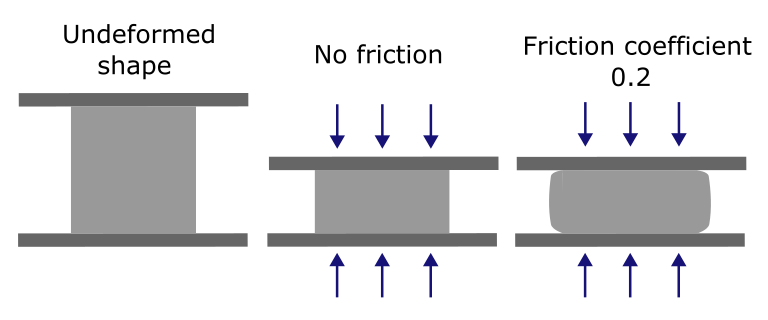
\includegraphics[width=10cm]{Images/chapter1/compressiondiag.png}%
       \caption{Uniaxial compression testing: Diagram of typical compression setup and influence of interface friction on the deformed specimen shape \cite{Bergström2015}.}%
       \label{fig:compressiondiag}%
\end{figure}

Drass M. et al. conducted a uniaxial compression test, showing that the lubrication was 
crucial for an homogenous stress and strain distribution. The specimen tested was made from Transparent Structural 
Silicone Adhesive (TSSA), a rubber-like material commonly used in laminated connections within glass structures.
In this study homogeneous and inhomogeneous experiments were performed, as the goal was to determine an 
experimental setup, which ensured an homogeneous stress and strain distributions for the identification of material parameters \cite{Drass2018}.

The specimen was compressed with perfect slippage, where the plates and the specimen were lubricated 
before testing to ensure a frictionless support. A constant speed of $v_{UC}=\SI[per-mode = symbol]{0.174}{\milli \m\per \minute}$
was used for this test with a saBesto HHS 5000 machine. The compression test were consucted until a strain $\epsilon=\SI{0.6}{}$ 
was reached, as the standard deviation for large compression strain ($\epsilon>\SI{0.5}{}$) was too large.
The test presented challenges in maintaining the lubrication throughout the test, as it tended to be 
pressed out between the test specimen and the pressure plates, resulting in a increased friction. 

The results of this experiment were processed to identify hyperelastic material parameters using standard 
fitting routines and inverse methods. The test suggested that only stress-strain response up to a strain value of 
$\epsilon=\SI{0.5}{}$ should be considered for the indentification of the TSSA material parameters, as 
the friction's impact can be neglected for smaller strains.\\

In comparison, for a biomaterials,e.g., human soft tissues, a compressive testing of cartilage was conducted by Griffin M. et al. 
This study aimed to provide a protocol were compressive and tensile properties of human soft tissues can be evaluated 
and characterized with minimal destruction. By understanding these material's properties and calculating the Young's 
elastic modulus, it would be possible to obtain a benchmark for creating suitable tissue-engineered substitutes \cite{Griffin2016}. 

The mechanical response of cartilage is highly dependant to the fluid's flow through the tissue. The methods for compression 
testing can vary with confined or unconfined specimen, and the most prevalent, indentantion (Fig. \ref{fig:compressiontypes}).
In the unconfined compression the cartilage is pressured using a non-porous plate onto a non-porous chamber, 
leading to a predominatly radial fluid flow. For the confined compression the sample was placed in a sealed, 
fluid-filled impermeable chamber and loaded with a porous plate, making the fluid flow restricted to a vertical direction.
Finally, the indentation testing employed a smaller indenter applied to the sample's surface perpendicularly, ensuring 
uniaxial compression and minimizing shear loading. All test were conducted in a 
hydrated environment and the cartilage was submerged in phosphate-buffered saline before and during the test to maintain 
the hydration. With the latest compression testing type it was possible to identify elastic and viscoleastic properties 
of the sample \cite{Griffin2016}.

\begin{figure}%
        \centering
       \quad
       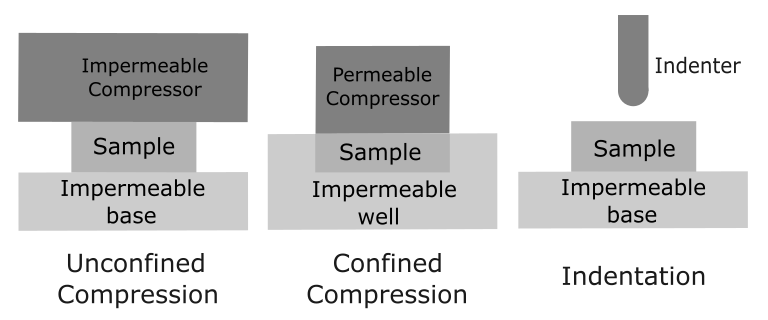
\includegraphics[width=10cm]{Images/chapter1/compressiontypes.png}%
       \caption{Uniaxial compression testing: Illustration of different compression methodologies for a cartilage specimen. Unconfined compression, confined compression and Indentation. \cite{Griffin2016}.}%
       \label{fig:compressiontypes}%
\end{figure}

%------------------------------------------------------------------------
\subsubsection*{Indentation}
Indentation testing, icluding micro and nanoindentation, is a popular method for characterizing 
the mechanical properties of soft materials \cite{Wu2016}. One of the main advantages of 
indentation testing is that it requires minimal sample preparation and it is often a 
nondestructive technique, which allows the preservation of the geometry and tissue's architecture \cite{Shi2019}.
Furthermore, indentation is useful where more traditional testing techniques such as 
uniaxial or biaxial testing, are not possible to employ, 
and can also be utilized to evaluate nonlinear properties, e.g., viscoplastic responses\cite{Bergström2015}.\\

Despite these advantages, there are some challenges when using indentation to 
characterize soft materials. First, a stress-strain response is difficult to
obtain due to the complex boundary conditions, which introduces an inverse problem 
for the identification of material parameters \cite{Shi2019}. Second, many of the current 
indentation configurations assume material isotropy, which may not be the case for biomaterials \cite{Feng2017}.
In addition, determining the mechanical properties of soft materials locally or at small scales is still difficult to achieve \cite{Zhang2014}.


The usual indentation testing setup is shown in Figure \ref{fig:Nanoindentation}, in this case a 
system applies a certain force to an attached indenter rod where and specific 
indenter tip. After the indenter tip goes to a determined displacement, 
it is possible to obtain a load-displacement curve.
The deformation can be measured through an capacitance gauge or also optically, via laser measurements \cite{Bergström2015}.

\begin{figure}[th]
        \centering
        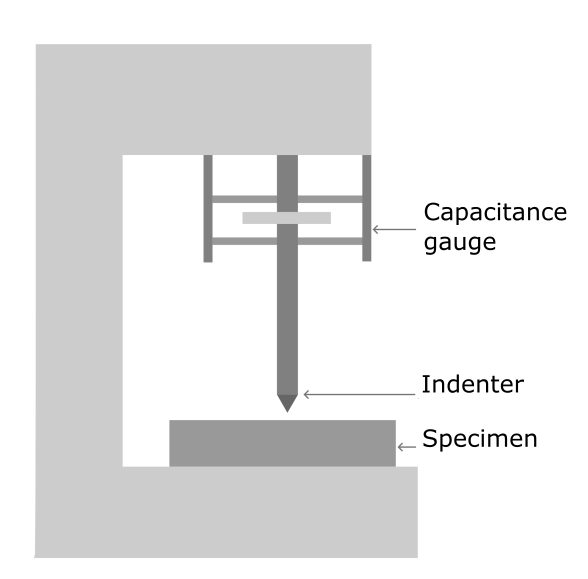
\includegraphics[width=7cm]{Images/nanoindentationbigletter}
        \caption[Nanoindentation]{Nanoindentation experiment setup diagram with an indenter tip attached to a rod and a polymer as specimen \cite{Bergström2015}.}
        \label{fig:Nanoindentation}
\end{figure}

In a study made by 

%-------------------------------------------------------------------------------------------------
\subsubsection*{Aspiration Experiment}

Tissue aspiration experiments introduces an aspiration tube which is put against the 
soft tissue, generating a vacuum. An advantageous feature of this experiment is that 
it can be perfomed in-vivo and ex-vivo.
With the help of a mirror placed next to aspiration 
hole, the reflection of the side-view of the tissue can be captured with a video camera.
This camera captures the images of the iluminated surface of the material and the 
aspiration pressure is captured through a sensor. Through this process the captured 
profile of the tissue is obtained and this can be used to characterize the deformation 
and analyze the viscoelastic properties of the soft tissue\cite{Kauer2002}.



%---------------------------------------------------------------------------------
\subsection{Material Modeling of Soft Materials}
 
Relevant papers tends to use hyperelastic models to represent soft materials as the viscoelasticity 
is usually neglected. 
% why do they use hyperelastic formulas? Why is it possible to neglect the viscoelasticity
%Revisar
Material model are very relevant for the simulation model (Kauer2002).
Soft tissues are approximated as near incompressible due to their highly water content.  
%viscoelastic example
For the aspiration experiment conducted by Kauer they used the following strain energy
function based on the model of Susanne and Bathe (SusanneandBAthe1987)
%Revisar


As derivative from this formula for the uteri metrial modeling the formula used was:

%---------------------------------------------------------------------------------
\subsection{Inverse Finite Element Method for Parameter Identification}

An inverse finite element (FE) approach requires usually a certain experimental model,
 which generates certain information e. g. load-displacement curve, and through 
a verified computational model match the given data curve to obtain further information 
of the material's behavior e. g., stress-strain curve.

Specially for nonlinear cases \cite{Husain2004}, where the complexity of the problems 
increases, and the interest is focused to generate an action which results in a 
certain output response, is where an inverse finite element approach can be helpful 
to discover a certain variable going from an ouput data. Through an iterative process it is 
possible to describe the material's behavior and validate the output data it 
through other established testing e. g., uniaxial testing.

Though this approach does not always give a hundred percent match in all obtain points 
or zones, it allows the researcher to understand the influences of certain parameters 
for the materials. This is specially useful for complex materials as biomaterials. 

Biomaterials, as mentioned previously, depends on multiple external factors, e.g., blood 
pressure, affected diseases and the their material properties is constantly changing. 
This issue does not allow the researcher to develop a proper material model which is 
usable for multiple use-cases. 

Therefore, the importance of the inverse element method as relevant key for estimating 
constantly changing parameters in soft materials.

For biomechanical models, where the models require knowledge from local properties \cite{Chai2013},
as the biomaterial is not isotropic; it is possible to identify a parameter e.g. Young's Modulus 
from a 3D model. The model can be matched to multiple experiments and multiple samples in different areas,
which allows a better representation of the material for further analysis.

The inverse FE approach can used by optimizing the searched parameter by matching the simulated data
to a section of a experimental curve and extending this process through some iterations. 
Nevertheless, it is important to clarify that this method also requires making assumptions to some values.
Furthermore, it is relevant to document these assumptions for the further analysis. 
With the combination of assumptions, experimental data, and a optimized and matched simulation curve, it
is possible to solve the complexity of biomechanical models.
 
In next sections some of the experimental models and the material models for bio and soft materials are 
going to be explained to get a further understanding in how is possible to get a realiable computational 
model for further reasearch

\subsubsection*{Synthetic Soft Materials}

Synthetics materials are commonly used to validate an inverse parameter identification process. 
Usually these synthetic, soft materials provide similar mechanical behavior to it's biomaterials 
counterparts. This characterization allows to validate a proposed inverse finite element approach process
before its applicatoin with a biomaterial, where the measurements to gather the experimental data are 
some in-vivo, and more challenging to recreate.


For example, Silgel, a very soft gel-like material \cite{Kauer2002} was used for the experimental 
validation of the inverse finite element method proposed, to characterized the tissue of 
a human uteri. In this work, the tensile behavior of the material was predicted through the 
parameters obtained in the aspiration method. The matching procedure is optimize through 
an objective function, which consists of the squared differences between the simulation 
and exprimental data. With an optimization algorithm an optimal set of the following parameters 
was found: the material parameters \(\mu_i\) [N/m\textsuperscript{2}] and the bulk Modulus
\(\kappa\) [N/m\textsuperscript{2}]. This method showed good prediction quality of the mentioned 
material parameters.

\subsubsection*{Biomaterials}
Biomaterials as mentioned before, represent a challenge due its difficult access and lesser replicability.
Therefore these materials are usually used for the experimetnal validation of a methd applied previously in 
synthetic materials. 
 Following the first example of the Silgel in the previous section, the inverse finite element parameter
 estimation is applied now on human uteri \cite{Kauer2002} through in vivo and ex vivo measurements of the human tissue of 
 different patients. It was mentioned, that in comparison from the silgel the uterus possesses a complex 
 multi layered structure with strongly anistropic and viscoelastic properties. Nevertheless, five 
 material parameters were determined, based on the strain energy function to model a human uterus (Yamada 1970).
Through the same inverse method applied with the synthetic material, the obtained parameters facilitated the prediction of stress-elongation curves for tensile experiments. The 
 resulting curves showed the difference of stiffness for in vivo and ex vivo measurements and the material 
 singurality for each uterus.


\subsection{Standard Verification and Validation for Computational Solid Mechanics (ASME)}
\subsubsection*{VV40}


%---------------------------------------------------------------------------------

\section{Overview}